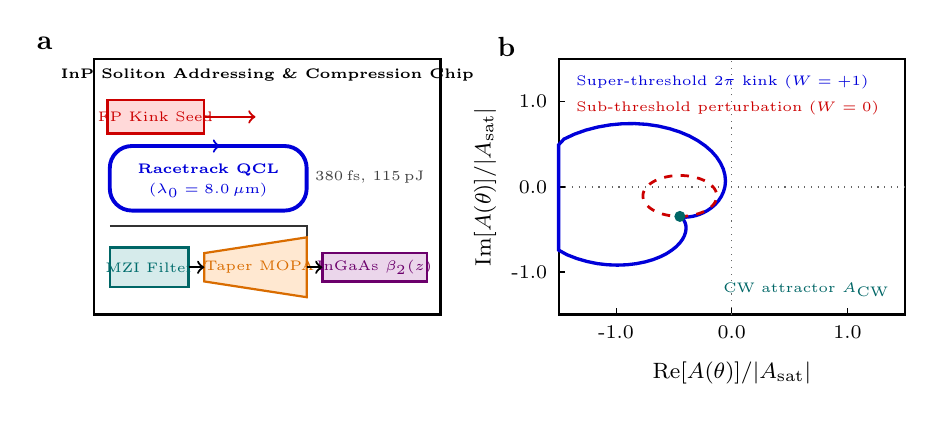
\begin{tikzpicture}[x=1cm,y=1cm,font=\footnotesize]
  % Panel a: Monolithic 4-Stage InP Photonic Chip Schematic
  \node[anchor=north west,font=\bfseries\normalsize] at (0.10,4.35) {a};
  \draw[thick] (0.95,0.70) rectangle (5.35,3.95);
  \node[font=\tiny\bfseries] at (3.15,3.74) {InP Soliton Addressing \& Compression Chip};

  % FP Phase-Kink Seed Injector
  \fill[red!15] (1.12,3.00) rectangle (2.35,3.42);
  \draw[red!80!black,thick] (1.12,3.00) rectangle (2.35,3.42);
  \node[font=\tiny,red!80!black] at (1.73,3.21) {FP Kink Seed};
  \draw[->,red!80!black,thick] (2.35,3.21) -- (3.00,3.21);

  % Unidirectional Racetrack QCL
  \draw[blue!85!black,line width=1.4pt,rounded corners=0.28cm] (1.15,2.02) rectangle (3.65,2.84);
  \node[font=\tiny\bfseries,blue!85!black] at (2.40,2.54) {Racetrack QCL};
  \node[font=\tiny,blue!85!black] at (2.40,2.28) {($\lambda_0=8.0\,\mu\mathrm{m}$)};
  \draw[->,blue!85!black,thick] (2.20,2.84) -- (2.55,2.84);

  % Output bus -> MZI CW Filter -> Flaring MOPA -> InGaAs Compressor
  \draw[thick,black!80] (1.15,1.82) -- (3.65,1.82) -- (3.65,1.32);
  \fill[teal!16] (1.15,1.05) rectangle (2.15,1.55);
  \draw[teal!80!black,thick] (1.15,1.05) rectangle (2.15,1.55);
  \node[font=\tiny,teal!85!black] at (1.65,1.30) {MZI Filter};

  \fill[orange!18] (2.35,1.12) -- (3.65,0.92) -- (3.65,1.68) -- (2.35,1.48) -- cycle;
  \draw[orange!85!black,thick] (2.35,1.12) -- (3.65,0.92) -- (3.65,1.68) -- (2.35,1.48) -- cycle;
  \node[font=\tiny,orange!85!black] at (3.05,1.30) {Taper MOPA};

  \fill[violet!16] (3.85,1.12) rectangle (5.18,1.48);
  \draw[violet!85!black,thick] (3.85,1.12) rectangle (5.18,1.48);
  \node[font=\tiny,violet!85!black] at (4.51,1.30) {InGaAs $\beta_2(z)$};

  \draw[->,thick] (2.15,1.30) -- (2.35,1.30);
  \draw[->,thick] (3.65,1.30) -- (3.85,1.30);
  \node[font=\tiny,black!75] at (4.45,2.45) {$380\,\mathrm{fs}$, $115\,\mathrm{pJ}$};

  % Panel b: Argand-Plane Topological Phase-Kink Trajectory
  \node[anchor=north west,font=\bfseries\normalsize] at (5.95,4.35) {b};
  \draw[thick] (6.85,0.70) rectangle (11.25,3.95);
  \foreach \v/\y in {-1.0/1.24, 0.0/2.32, 1.0/3.41} {
    \draw (6.85,\y) -- (6.93,\y);
    \node[left,font=\scriptsize] at (6.83,\y) {\v};
  }
  \foreach \xval/\xpos in {-1.0/7.58, 0.0/9.05, 1.0/10.52} {
    \draw (\xpos,0.70) -- (\xpos,0.78);
    \node[below,font=\scriptsize] at (\xpos,0.68) {\xval};
  }
  \node[below,font=\footnotesize] at (9.05,0.22) {$\mathrm{Re}[A(\theta)]/|A_{\mathrm{sat}}|$};
  \node[rotate=90,above,font=\footnotesize] at (6.18,2.32) {$\mathrm{Im}[A(\theta)]/|A_{\mathrm{sat}}|$};

  % Origin crosshairs (phase singularity W=1)
  \draw[dotted,black!60] (6.85,2.32) -- (11.25,2.32);
  \draw[dotted,black!60] (9.05,0.70) -- (9.05,3.95);

  \draw[blue!85!black,line width=1.2pt] (8.390,1.946) -- (8.393,1.945) -- (8.402,1.943) -- (8.418,1.940) -- (8.440,1.938) -- (8.469,1.937) -- (8.505,1.940) -- (8.546,1.946) -- (8.591,1.956) -- (8.640,1.972) -- (8.691,1.994) -- (8.742,2.022) -- (8.792,2.057) -- (8.839,2.098) -- (8.882,2.147) -- (8.917,2.201) -- (8.945,2.262) -- (8.963,2.327) -- (8.969,2.397) -- (8.962,2.471) -- (8.942,2.546) -- (8.907,2.622) -- (8.858,2.698) -- (8.793,2.772) -- (8.713,2.842) -- (8.619,2.907) -- (8.511,2.967) -- (8.390,3.018) -- (8.259,3.060) -- (8.118,3.093) -- (7.970,3.115) -- (7.816,3.125) -- (7.659,3.123) -- (7.502,3.108) -- (7.347,3.081) -- (7.196,3.042) -- (7.052,2.991) -- (6.918,2.928) -- (6.850,2.855) -- (6.850,2.773) -- (6.850,2.682) -- (6.850,2.584) -- (6.850,2.482) -- (6.850,2.375) -- (6.850,2.267) -- (6.850,2.158) -- (6.850,2.051) -- (6.850,1.946) -- (6.850,1.846) -- (6.850,1.752) -- (6.850,1.665) -- (6.850,1.587) -- (6.850,1.518) -- (6.957,1.459) -- (7.081,1.411) -- (7.209,1.374) -- (7.339,1.347) -- (7.469,1.332) -- (7.597,1.327) -- (7.720,1.332) -- (7.838,1.346) -- (7.948,1.368) -- (8.049,1.397) -- (8.140,1.433) -- (8.220,1.473) -- (8.288,1.517) -- (8.345,1.563) -- (8.390,1.610) -- (8.424,1.656) -- (8.448,1.702) -- (8.462,1.745) -- (8.468,1.785) -- (8.467,1.822) -- (8.461,1.853) -- (8.450,1.880) -- (8.437,1.902) -- (8.424,1.920) -- (8.411,1.932) -- (8.400,1.940) -- (8.393,1.945) -- (8.390,1.946);
  \draw[red!80!black,dashed,line width=1.0pt] (8.390,1.946) -- (8.427,1.947) -- (8.463,1.949) -- (8.500,1.953) -- (8.535,1.959) -- (8.570,1.966) -- (8.603,1.974) -- (8.635,1.984) -- (8.666,1.995) -- (8.695,2.008) -- (8.722,2.022) -- (8.747,2.037) -- (8.770,2.053) -- (8.790,2.070) -- (8.808,2.088) -- (8.824,2.106) -- (8.836,2.125) -- (8.846,2.145) -- (8.854,2.165) -- (8.858,2.185) -- (8.859,2.206) -- (8.858,2.226) -- (8.854,2.247) -- (8.846,2.267) -- (8.836,2.286) -- (8.824,2.305) -- (8.808,2.324) -- (8.790,2.342) -- (8.770,2.359) -- (8.747,2.375) -- (8.722,2.390) -- (8.695,2.404) -- (8.666,2.416) -- (8.635,2.428) -- (8.603,2.437) -- (8.570,2.446) -- (8.535,2.453) -- (8.500,2.459) -- (8.463,2.463) -- (8.427,2.465) -- (8.390,2.466) -- (8.353,2.465) -- (8.317,2.463) -- (8.280,2.459) -- (8.245,2.453) -- (8.210,2.446) -- (8.177,2.437) -- (8.145,2.428) -- (8.114,2.416) -- (8.085,2.404) -- (8.058,2.390) -- (8.033,2.375) -- (8.010,2.359) -- (7.990,2.342) -- (7.972,2.324) -- (7.956,2.305) -- (7.944,2.286) -- (7.934,2.267) -- (7.926,2.247) -- (7.922,2.226) -- (7.921,2.206) -- (7.922,2.185) -- (7.926,2.165) -- (7.934,2.145) -- (7.944,2.125) -- (7.956,2.106) -- (7.972,2.088) -- (7.990,2.070) -- (8.010,2.053) -- (8.033,2.037) -- (8.058,2.022) -- (8.085,2.008) -- (8.114,1.995) -- (8.145,1.984) -- (8.177,1.974) -- (8.210,1.966) -- (8.245,1.959) -- (8.280,1.953) -- (8.317,1.949) -- (8.353,1.947) -- (8.390,1.946);
  \fill[teal!80!black] (8.390,1.946) circle (2.0pt);

  \node[anchor=north west,font=\tiny,blue!85!black] at (6.95,3.86) {Super-threshold $2\pi$ kink ($W=+1$)};
  \node[anchor=north west,font=\tiny,red!80!black] at (6.95,3.54) {Sub-threshold perturbation ($W=0$)};
  \node[anchor=south east,font=\tiny,teal!80!black] at (11.18,0.80) {CW attractor $A_{\mathrm{CW}}$};
\end{tikzpicture}
